\documentclass[11pt,aspectratio=1610,xcolor=dvipsnames]{beamer}

\usetheme[
    background=light,
    numbering=fraction,
    block=fill,
    progressbar=frametitle
]{metropolis}

\usepackage{physics}
\usepackage{bbm}
\usepackage[most]{tcolorbox}
\usepackage{tikz}
\usetikzlibrary{arrows}
% \colorlet{LightLavender}{Lavender!40!}
\newtcolorbox{prob}{colback=green!5!white,colframe=green!75!black}
\usefonttheme[onlymath]{serif}
\newcommand{\R}{\mathbb{R}}
\newcommand{\defeq}{\stackrel{\text{\tiny def}}{=}}


\newcommand{\problemstatement}{Does the topology on Minkowski space agree with the ``metric topology'' induced by the metric $\eta_{\mu\nu} = \smqty[-1 & & &  \\ & \phantom{+}1 & & \\ & & \phantom{+}1 & \\ & & & \phantom{+}1]$?}
\newcommand{\problemstatementtwo}{What is the topology on $\R^{1,3}$ with the metric $\eta_{\mu\nu} = \smqty[-1 & & &  \\ & \phantom{+}1 & & \\ & & \phantom{+}1 & \\ & & & \phantom{+}1]$?}
\title{General Relativity Exam Problem 3}
\date{Sep 30, 2021}
\author{Nate Stemen (he/they)}
\institute{AMATH 875}


\begin{document}

\maketitle

\begin{frame}
	\begin{figure}
		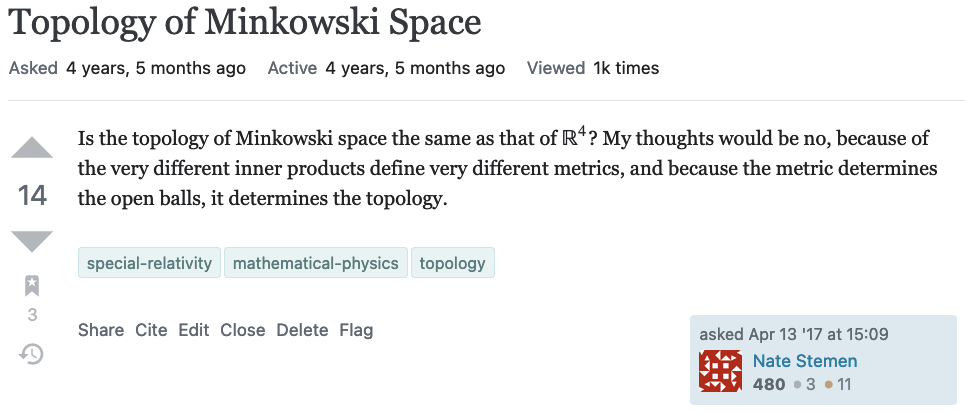
\includegraphics[width=.8\textwidth]{physSE.png}
	\end{figure}
\end{frame}

\begin{frame}{Problem Statement}
	\large
	\begin{prob}
		\problemstatement
	\end{prob}
	\begin{prob}
		\problemstatementtwo
	\end{prob}
\end{frame}

\begin{frame}{What's Minkowski space?}
	\begin{center}
		\huge $\R\times \R^3$ equipped with the metric $\eta_{\mu\nu} = \smqty[-1 & & &  \\ & \phantom{+}1 & & \\ & & \phantom{+}1 & \\ & & & \phantom{+}1]$.
	\end{center}
\end{frame}

\begin{frame}{Recall: What's the metric tensor?}
	\begin{definition}
		Let $M$ be a smooth manifold.
		The metric tensor $g$ is a rank $(0, 2)$ tensor field that is
		\begin{itemize}
			\item bilinear
			\item symmetric
			\item nondegenerate
		\end{itemize}
	\end{definition}
	\pause
	Another way of viewing $g$ is that for each $p\in M$ we have a nondegenerate symmetric bilinear form $g_p: T_p(M)\times T_p(M) \to \R$ that varies smoothly as we move $p$.
\end{frame}

\begin{frame}{What happens when $T_p(M) \cong M$ for all $p$?}
	\begin{itemize}
		\item If $T_p(M) \cong M$ then our metric tensor is extended to all of $M$: $g_p: M \times M \to \R$
		\item Can drop subscript $p$
		\item Hence we have a nondegenerate, symmetric bilinear form on all of $M$
		\item Sounds like an inner product?
		\item Can then define a norm: $\norm{u}_g \defeq g(u, u)$
		\item Can then define a metric: $d_{\norm{\cdot}_g}(x, y) \defeq \norm{x - y}_g$
	\end{itemize}
\end{frame}

\begin{frame}{What is the metric topology?}
	\begin{definition}[Metric Space]
		A \emph{metric space} is a pair $(M, d)$ where $M$ is a set, and $d$ is a function $d: M \times M \to \R$ satisfying
		\begin{itemize}
			\item $d(x, y) = 0$ if and only if $x = y$,
			\item $d(x, y) = d(y, x)$, and
			\item $d(x, z) \leq d(x, y) + d(y, z)$.
		\end{itemize}
	\end{definition}
	\pause
	\begin{definition}[Metric Topology]
		For any $x\in M$ and $r > 0$, we define the open ball of radius $r$ to be
		\begin{equation*}
			B(x\,; r) = \qty{y\in M : d(x, y) < r}.
		\end{equation*}
		These open balls form a base for a topology.
	\end{definition}
	$\R^n$ (the set) taken with the open balls generated by the Euclidean metric form the standard topology for $\R^n$ (the topological space).
\end{frame}

\begin{frame}{Open Balls in Minkowski Space}
	\begin{center}
		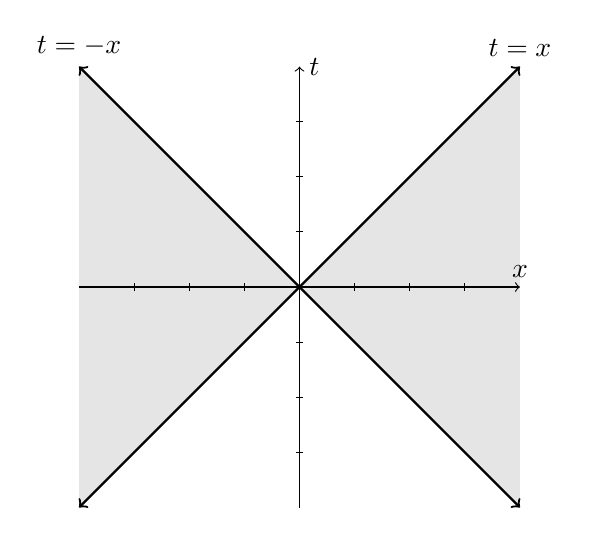
\begin{tikzpicture}[scale=.7]
			\fill[fill=gray!20] (0,0) -- (4,4) -- (4,-4) -- cycle;
			\fill[fill=gray!20] (0,0) -- (-4,4) -- (-4,-4) -- cycle;

			\draw[->] (0,-4) -- (0,4) node[right](tline) {$t$};
			\draw[->] (-4,0) -- (4,0) node[above](xline) {$x$};
			\foreach \x in {-3,-2,-1,1,2,3}
			\draw (\x,2pt) -- (\x,-2pt);
			\foreach \y in {-3,-2,-1,1,2,3}
			\draw (2pt,\y) -- (-2pt,\y);

			\draw[<->,thick] (-4,-4) -- (4,4) node[above] {$t = x$};
			\draw[<->,thick] (4,-4) -- (-4,4) node[above] {$t = -x$};
		\end{tikzpicture}
	\end{center}
\end{frame}

\begin{frame}
	\begin{figure}
		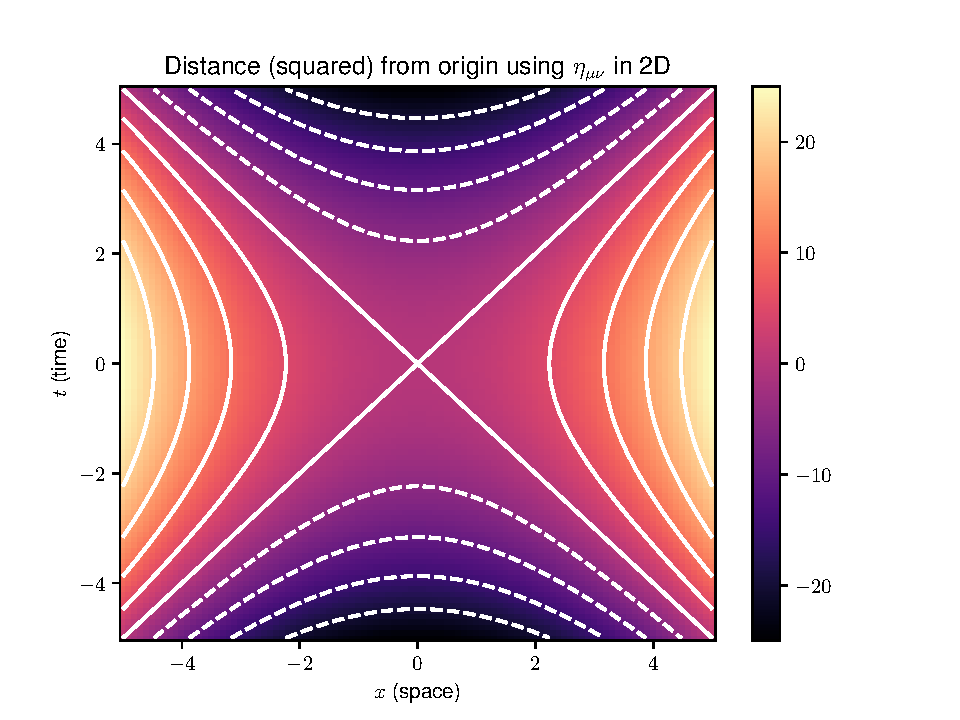
\includegraphics[width=0.8\textwidth]{contour.pdf}
	\end{figure}
\end{frame}

\begin{frame}{$\eta_{\mu\nu}$ isn't a proper inner product}
	\begin{itemize}[<+->]
		\item $\eta_{\mu\nu}$ isn't a proper inner product because it's not positive definite!
		      \begin{itemize}
			      \item $\eta(\smqty[t \\ x], \smqty[\tilde{t} \\ \tilde{x}]) = -(t - \tilde{t})^2 + (x - \tilde{x})^2$ can be negative
		      \end{itemize}
		\item I have no idea of the open balls induced by $\eta$ \emph{can} form a base for a topology
		\item I \emph{think} we just take the topology of $\R^{1,3}$ to be that of standard $\R^4$ because of this wonkyness
		\item After all one usually specifies
		      \begin{equation*}
			      \text{set} \longrightarrow \text{topology} \longrightarrow \text{differentiable structure} \longrightarrow \cdots
		      \end{equation*}
		      so the topology is set from the beginning
		\item I thought the metric might have to coincide with the topology, but perhaps not
	\end{itemize}
\end{frame}
\end{document}
